\documentclass[11pt]{extarticle} 
\usepackage{unicode-math}
\usepackage{mathrsfs}
\usepackage{amsthm,graphicx,xcolor,natbib,enumitem,booktabs,tabularx}
\usepackage[paperwidth=126mm, paperheight=96mm, top=5mm, bottom=5mm, right=5mm, left=5mm]{geometry}
\pagenumbering{gobble}

\usepackage[BoldFont,SlantFont]{xeCJK}  
\xeCJKsetemboldenfactor{2}
\setCJKmainfont{cwTeX Q Yuan Medium}

\usepackage{hyperref}
\hypersetup{
    colorlinks,
    linkcolor={red!50!black},
    citecolor={blue!60!black},
    urlcolor={blue!60!black}
}

\newcommand{\ds}{\displaystyle}
\newcommand{\ie}{\;\Longrightarrow\;}
\newcommand{\ifff}{\;\Longleftrightarrow\;}
\newcommand{\mi}{\mathrm{i}}
\DeclareMathOperator*{\dom}{dom}
\DeclareMathOperator*{\codom}{codom}
\DeclareMathOperator*{\ran}{ran}
\newcommand{\floor}[1]{\lfloor #1 \rfloor}
\newcommand{\ceil}[1]{\lceil #1 \rceil}
\newcommand{\Set}[2]{\big\{ \ #1\ \big|\ #2\ \big\}}
\newcommand{\pdiff}[2]{\frac{\partial\hfil#1\hfil}{\partial #2}}

\DeclareMathOperator\prb{{\sf P}}
\DeclareMathOperator\expc{{\sf E}}
\DeclareMathOperator\var{var}
\DeclareMathOperator\cov{cov}
\DeclareMathOperator*{\argmax}{\arg\!\max}
\DeclareMathOperator*{\argmin}{\arg\!\min}
\DeclareMathOperator*{\im}{Im}
\DeclareMathOperator*{\re}{Re}
\DeclareMathOperator*{\conv}{conv}
\DeclareMathOperator*{\proj}{proj}
\DeclareMathOperator*{\tr}{tr}
\DeclareMathOperator*{\diag}{diag}
\DeclareMathOperator*{\epi}{epi}
\DeclareMathOperator*{\dist}{dist}
\DeclareMathOperator*{\inte}{int}
\DeclareMathOperator*{\relint}{relint}

\theoremstyle{definition}
\newtheorem*{dfn}{Definition}
\newtheorem*{prp}{Property}
\newtheorem*{thm}{Theorem}
\newtheorem*{ex}{Example}
\newtheorem*{sol}{Solution}
\newtheorem*{prf}{Proof}

\newcommand\scalemath[2]{\scalebox{#1}{\mbox{\ensuremath{\displaystyle #2}}}}

\begin{document}
\title{\texorpdfstring{\vspace{15mm} Operations Research\\ 07. Duality}{Operations Research\\ 07. Duality}} 
\author{}
\date{}
\maketitle
\newpage

\section*{Lagrangian}

\begin{itemize}
  \item {\bf standard form problem} (not necessarily convex)
    \begin{align*}
      \text{minimize}\quad &f_0(x) \\
      \text{subject to}\quad &f_i(x)\leqslant 0, \quad i = 1, 2,\,\ldots,\,m \\
      \qquad\qquad &h_i(x) = 0, \quad i = 1, 2,\,\ldots,\,p 
    \end{align*}
    variable $x\in\mathbb{R}^n$, domain $\mathcal{D}$, optimal value $p^\star$
  \item {\bf Lagrangian} $L:\mathbb{R}^n\times\mathbb{R}^m\times\mathbb{R}^p\to\mathbb{R}$, with $\dom f = \mathcal{D}\times\mathbb{R}^m\times\mathbb{R}^p$
    \begin{align*}
      L(x,\lambda,\nu) = f_0(x) + \sum_{i=1}^m\lambda_i f_i(x) + \sum_{i=1}^p\nu_i h_i(x)
    \end{align*}
    \begin{itemize}
      \item weighted sum of objective and constraints 
      \item $\lambda_i$ is Lagrange multiplier associated with $\ds f_i(x)\leqslant 0$
      \item $\nu_i$ is Lagrange multiplier associated with $\ds h_i(x) = 0$
    \end{itemize}
\end{itemize}

\newpage

\section*{Lagrange Dual Function}

\begin{itemize}
  \item {\bf Lagrange dual function}: $g:\mathbb{R}^m\times\mathbb{R}^p\to\mathbb{R}$, 
    \begin{align*}
      g(\lambda,\nu) =\inf_{x\in\mathcal{D}}L(x,\lambda,\nu) = \inf_{x\in\mathcal{D}}\bigg(f_0(x) + \sum_{i=1}^m\lambda_i f_i(x) + \sum_{i=1}^p\nu_i h_i(x)\bigg)
    \end{align*}
  \item $g$ is concave, can be $-\infty$ for some $\lambda,\,\nu$
  \item {\bf lower bound property}: $g(\lambda,\nu) \leqslant p^\star$ if $\lambda\succcurlyeq 0$
  \item proof: if $\ds\widetilde{x}$ is feasible and $\lambda\succcurlyeq 0$, then
    \begin{align*}
      f_0(\widetilde{x})\geqslant L(\widetilde{x},\lambda,\nu)\geqslant\inf_{x\in\mathcal{D}}L(x,\lambda,\nu) = g(\lambda,\nu)
    \end{align*}
  \item minimizing over all feasible $\ds\widetilde{x}$ gives $\ds p^\star\geqslant g(\lambda,\nu)$
\end{itemize}

\newpage

\section*{Least-Norm Solution of Linear Equations}
\begin{align*}
  \text{minimize}\quad & x^\top x \\
  \text{subject to}\quad & A\,x = b
\end{align*}
\begin{itemize}
  \item Lagrangian is $\ds L(x,\,\nu) = x^\top x + \nu^\top(A\,x - b)$
  \item to minimize $L$ over $x$, set gradient equal to zero:
    \begin{align*}
      \nabla_x L(x,\,\nu) = 2 x + A^\top\nu = 0\ie x = -\frac{1}{2}A^\top\nu
    \end{align*}
  \item plug $x$ into $L$ to obtain
    \begin{align*}
      g(\nu) = L\Big(-\frac{1}{2}A^\top\nu,\,\nu\Big) = -\frac{1}{4}\nu^\top AA^\top\nu - b^\top\nu
    \end{align*}
  \item lower bound property: $\ds p^\star\geqslant -\frac{1}{4}\nu^\top AA^\top\nu - b^\top\nu,\;\forall\,\nu$
\end{itemize}

\newpage

\section*{Least-Norm Solution of Linear Equations}
\begin{align*}
  \text{minimize}\quad & x^\top x \\
  \text{subject to}\quad & A\,x = b
\end{align*}
\begin{itemize}
  \item Lagrangian is $\ds L(x,\,\nu) = x^\top x + \nu^\top(A\,x - b)$
  \item to minimize $L$ over $x$, set gradient equal to zero:
    \begin{align*}
      \nabla_x L(x,\,\nu) = 2 x + A^\top\nu = 0\ie x = -\frac{1}{2}A^\top\nu
    \end{align*}
  \item plug $x$ into $L$ to obtain
    \begin{align*}
      g(\nu) = L\Big(-\frac{1}{2}A^\top\nu,\,\nu\Big) = -\frac{1}{4}\nu^\top AA^\top\nu - b^\top\nu
    \end{align*}
  \item lower bound property: $\ds p^\star\geqslant -\frac{1}{4}\nu^\top AA^\top\nu - b^\top\nu,\;\forall\,\nu$
\end{itemize}

\newpage

\section*{Standard Form LP}
\begin{align*}
  \text{minimize}\quad & c^\top x \\
  \text{subject to}\quad & A\,x = b, \quad x\succcurlyeq 0
\end{align*}
\begin{itemize}
  \item Lagrangian is 
    \begin{align*}
      \ds L(x,\lambda,\nu) = c^\top x - \lambda^\top x + \nu^\top(A\,x - b) = -b^\top\nu + (c + A^\top\nu - \lambda)^\top x
    \end{align*}
  \item $L$ is affine in $x$, so 
    \begin{align*}
      g(\lambda, \nu) = \inf_{x}\,L(x,\lambda,\nu) = \begin{cases}-b^\top\nu & A^\top\nu - \lambda + c = 0 \\ -\infty & \text{otherwise}\end{cases}
    \end{align*}
  \item $g$ is linear on affine domain $\ds\{(\lambda,\,\nu)\;|\;A^\top\nu - \lambda + c = 0\}$, hence concave
  \item lower bound property: $\ds p^\star\geqslant -b^\top\nu$ if $\ds A^\top\nu + c\succcurlyeq 0$
\end{itemize}

\newpage

\section*{Lagrange Dual and Conjugate Function}
\begin{align*}
  \text{minimize}\quad & f_0(x) \\
  \text{subject to}\quad & A\,x\preccurlyeq b,\quad C\,x = d
\end{align*}
\begin{itemize}
  \item dual function 
    \begin{align*}
      g(\lambda, \nu) &= \inf_{x\in\dom{f_0}}\Big(f_0(x) + (A^\top\lambda + C^\top\nu)^\top x - b^\top\lambda - d^\top\nu\Big) \\
                      &= -f_0^\star(-A^\top\lambda - C^\top\nu) - b^\top\lambda - d^\top\nu
    \end{align*}
    where $\ds f_0^\star(y)\equiv\sup_{x\in\dom f_0} y^\top x - f_0(x)$ is {\bf conjugate} of $f_0$
  \item simplifies derivation of dual if conjugate of $f_0$ is known
  \item {\bf example: entropy maxmization}
    \begin{align*}
      f_0(x) = \sum_{i = 1}^n x_i\log x_i, \qquad f_0^\star(y) = \sum_{i = 1}^n e^{y_i - 1}
    \end{align*}
\end{itemize}

\newpage

\section*{The Lagrange Dual Problem}
\begin{align*}
  \text{maximize}\quad & g(\lambda,\,\nu) \\
  \text{subject to}\quad & \lambda\succcurlyeq 0
\end{align*}
\begin{itemize}
  \item find best lower bound on $\ds p^\star$, obtained from Lagrange dual function
  \item a convex optimization problem, even if original {\bf primal} problem is not
  \item dual optimal value denoted by $\ds d^\star$
  \item $\lambda$, $\nu$ are dual feasible if $\ds\lambda\succcurlyeq 0$, $\ds(\lambda,\,\nu)\in\dom g$
  \item often simplified by making implicit constraint $\ds (\lambda,\,\nu)\in\dom g$ explicit
\end{itemize}

\newpage

\section*{Example: Standard Form LP}
\begin{itemize}
  \item primal standard form LP
    \begin{align*}
      \text{minimize}\quad & c^\top x \\
      \text{subject to}\quad & A\,x = b,\quad x\succcurlyeq 0 
    \end{align*}
  \item dual problem 
    \begin{align*}
      \text{maximize}\quad & g(\lambda,\,\nu) \\
      \text{subject to}\quad & \lambda\succcurlyeq 0 
    \end{align*}
    with $\ds g(\lambda,\,\nu) = \begin{cases} -b^\top\nu & \text{if } A^\top\nu - \lambda + c = 0 \\ -\infty & \text{otherwise} \end{cases}$
  \item make implicit constraint explicit: eliminate $\lambda$ to obtain transformed dual problem
    \begin{align*}
      \text{maximize}\quad & -b^\top\nu \\
      \text{subject to}\quad & A^\top\nu + c \succcurlyeq 0 
    \end{align*}
\end{itemize}

\newpage

\section*{Equality Constrained Norm Minimization}
%\vspace{-3mm}
\begin{align*}
  \text{minimize}\quad & \|x\| \\
  \text{subject to}\quad & A\,x = b 
\end{align*}
\begin{itemize}%\setlength\itemsep{0em}
  \item dual function is \\
    \begin{align*}
      g(\nu) &= \inf_x \big(\|x\| - \nu^\top A\,x + b^\top\nu\big) = \begin{cases} b^\top\nu & \|A^\top\nu\|_\star\leqslant 1 \\ -\infty & \text{otherwise} \end{cases}
    \end{align*}
    where $\ds\|\nu\|_\star = \sup_{\|u\|\leqslant 1}u^\top\nu$ is dual norm of $\|\cdot\|$
  \item lower bound property: $p^\star\geqslant b^\top\nu$ if $\ds\|A^\top\nu\|_\star\leqslant 1$
\end{itemize}

\newpage

\section*{Two-Way Partitioning}
\vspace{-3mm}
\begin{align*}
  \text{minimize}\quad & x^\top Wx \\
  \text{subject to}\quad & x_i^2 = 1, \quad i = 1, 2,\,\ldots,\,n 
\end{align*}
\begin{itemize}\setlength\itemsep{0em}
  \item a nonconvex problem; feasible set contains $2^n$ discrete points
  \item interpretation: partition $\{1, 2, \ldots, n\}$ into two sets encoded as $x_i = 1$ and $x_i = -1$
  \item $W_{ij}$: cost of assigning $i$, $j$ to the same set\\
        $-W_{ij}$: cost of assigning $i$, $j$ to different sets
  \item dual function is \\
    \scalebox{0.95}{\parbox{\linewidth}{%
    \begin{align*}
      g(\nu) &= \inf_x \Big(x^\top Wx + \sum_i\nu_i(x_i^2 - 1)\Big) = \inf_x\big(x^\top(W + \diag\nu)x - \symbfup{1}^\top\nu\big) \\ &= \begin{cases} -\symbfup{1}^\top\nu & \text{if } W + \diag\nu\succcurlyeq 0 \\ -\infty & \text{otherwise} \end{cases}
    \end{align*}
    }}
    \vspace{-3mm}
  \item lower bound property: $p^\star\geqslant -\symbfup{1}^\top\nu$ if $W + \diag\nu\succcurlyeq 0$
\end{itemize}

\newpage

\section*{Weak and Strong Duality}

\begin{itemize}
  \item {\bf weak duality}: $\ds d^\star\leqslant p^\star$
    \begin{itemize}
      \item always holds for convex and nonconvex problems 
      \item can be used to find nontrivial lower bounds for hard problems, e.g. solving the SDP
        \begin{align*}
          \text{maximize}\quad & -\symbfup{1}^\top\nu \\
          \text{subject to}\quad & W + \diag(\nu)\succcurlyeq 0 
        \end{align*}
        gives a lower bound for two-way partitioning problem
    \end{itemize}
  \item {\bf strong duality}: $\ds d^\star = p^\star$
    \begin{itemize}
      \item does not hold in general 
      \item (usually) holds for convex problems
      \item conditions that guarantee strong duality in convex problems are called {\bf constraint qualifications}
    \end{itemize}
\end{itemize}

\newpage

\section*{Slater's Constraint Qualification}
strong duality holds for a convex problem
\begin{align*}
  \text{maximize}\quad & f_0(x) \\
  \text{subject to}\quad &f_i(x)\leqslant 0, \quad i = 1, 2,\,\ldots,\,m \\
  \qquad\qquad & A\, x = b
\end{align*}
if it is {\bf strictly feasible}, i.e. $\ds\exists\,x\in\inte\mathcal{D}$ with $\ds f_i(x) < 0$, $\ds i = 1, 2,\,\ldots,\,m$, $A\,x = b$  
\begin{itemize}
  \item also guarantees that the dual optimum is attained (if $\ds p^\star > -\infty$)
  \item can be sharpened, e.g.
    \begin{itemize}
      \item can replace $\ds\inte\mathcal{D}$ with $\ds\relint\mathcal{D}$ (interior relative to affine hull)
      \item linear inequalities do not need to hold with strict inequality
    \end{itemize}
  \item there are many other types of constraint qualifications
\end{itemize}

\newpage

\section*{Inequality Form LP}

\begin{itemize}\setlength\itemsep{0em}
  \item {\bf primal problem}
    \begin{align*}
      \text{minimize}\quad & c^\top x \\
      \text{subject to}\quad & A\,x \preccurlyeq b 
    \end{align*}
  \item {\bf dual function} 
    \begin{align*}
      g(\lambda,\,\nu) = \inf_x\big((c + A^\top\lambda)^\top x - b^\top\lambda\big) = \begin{cases} -b^\top\lambda & \text{if } A^\top\lambda + c = 0 \\ -\infty & \text{otherwise} \end{cases}
    \end{align*}
  \item {\bf dual problem}
    \begin{align*}
      \text{maximize}\quad & -b^\top\lambda \\
      \text{subject to}\quad & A^\top\lambda + c = 0, \quad \lambda\succcurlyeq 0 
    \end{align*}
  \item from the sharpened Slater's condition: $p^\star = d^\star$ if the primal problem is feasible
  \item in fact $p^\star = d^\star$ except when primal and dual are both infeasible
\end{itemize}

\newpage

\section*{Quadratic Program}

\begin{itemize}\setlength\itemsep{0em}
  \item {\bf primal problem} (assume $\ds P\in\mathsf{S}^n_{++}$)
    \begin{align*}
      \text{minimize}\quad & x^\top P\,x \\
      \text{subject to}\quad & A\,x \preccurlyeq b 
    \end{align*}
  \item {\bf dual function} 
    \begin{align*}
      g(\lambda) = \inf_x\big(x^\top P\,x + \lambda^\top(A\,x - b)\big) = -\frac{1}{4}\lambda^\top A P^{-1} A^\top\lambda - b^\top\lambda
    \end{align*}
  \item {\bf dual problem}
    \begin{align*}
      \text{maximize}\quad & -\frac{1}{4}\lambda^\top A P^{-1} A^\top\lambda - b^\top\lambda \\
      \text{subject to}\quad & \lambda\succcurlyeq 0 
    \end{align*}
  \item from the sharpened Slater's condition: $p^\star = d^\star$ if the primal problem is feasible
  \item in fact $p^\star = d^\star$ always
\end{itemize}

\newpage

\section*{Geometric Interpretation}

\begin{itemize}\setlength\itemsep{0em}
  \item for simplicity, consider problem with one constraint $\ds f_1(x)\leqslant 0$
  \item $\ds\mathcal{G} = \{(f_1(x),\,f_0(x))\;|\;x\in\mathcal{D}\}$ is set of achievable (constraint, objective) values
  \item {\bf interpretation of dual function}: $\ds g(\lambda) = \inf_{(u, t)\in\mathcal{G}} (\lambda u + t)$
    %\vspace{-3mm}
    \begin{figure}[!htbp]
      \centering
      \includegraphics[scale=0.6,page=3]{fig/05.pdf}
      \includegraphics[scale=0.6,page=4]{fig/05.pdf}
      %\caption{$y = \sin x$,$y = \sin^{-1} x$}
    \end{figure}
  \item $\ds\lambda u + t = g(\lambda)$ is (non-vertical) supporting hyperplane to $\mathcal{G}$
  \item hyperplane intersects $t$-axis at $t = g(\lambda)$
\end{itemize}

\newpage

\section*{Epigraph Variation}

\begin{itemize}\setlength\itemsep{0em}
  \item same with $\ds\mathcal{G}$ replaced with 
    \begin{align*}
      \mathcal{A} = \{(u,\,t)\;|\; f_1(x)\leqslant u,\,f_0(x)\leqslant t\;\,\text{for some}\;x\in\mathcal{D}\}
    \end{align*}
    \vspace{-2em}
    \begin{figure}[!htbp]
      \centering
      \includegraphics[scale=0.6,page=5]{fig/05.pdf}
    \end{figure}
    \vspace{-2em}
  \item strong duality holds if there is a non-vertical supporting hyperplane to $\mathcal{A}$ at $\ds (0, p^\star)$
  \item for convex problem, $\mathcal{A}$ is convex, hence has supporting hyperplane at $\ds (0, p^\star)$
  \item Slater's condition: if there exist $\ds(\widetilde{u},\,\widetilde{t})\in\mathcal{A}$ with $\ds\widetilde{u} < 0$, then supporting hyperplane at $\ds(0, p^\star)$ must be non-vertical
\end{itemize}

\newpage

\section*{Complementary Slackness}
\begin{itemize}
  \item assume strong duality holds, $\ds x^\star$ is primal optimal, $\ds(\lambda^\star,\nu^\star)$ is dual optimal
    \begin{align*}
      f_0(x^\star) = g(\lambda^\star, \nu^\star) &= \inf_{x}\bigg(f_0(x) + \sum_{i=1}^m\lambda_i^\star f_i(x) + \sum_{i=1}^p\nu_i^\star h_i(x)\bigg) \\
      &\leqslant f_0(x^\star) + \sum_{i=1}^m\lambda_i^\star f_i(x^\star) + \sum_{i=1}^p\nu_i^\star h_i(x^\star) \\
      &\leqslant f_0(x^\star)
    \end{align*}
  \item hence the two inequalities hold with equality
  \item $x^\star$ minimizes $L(x,\lambda^\star,\nu^\star)$
  \item $\ds\lambda_i^\star f_i(x^\star) = 0$, $\ds i = 1, 2,\,\ldots,\,m$: (known as {\bf complementary slackness})
    \begin{align*}
      \lambda_i^\star > 0\ie f_i(x^\star) = 0, \qquad f_i(x^\star) < 0\ie \lambda_i^\star = 0
    \end{align*}
\end{itemize}

\newpage

\section*{Karush-Kuhn-Tucker (KKT) Conditions}
KKT conditions (for a problem with differentiable $f_i$, $h_i$) are
\begin{enumerate}\setlength\itemsep{0em}
  \item primal constraints:
    \begin{align*}
      &f_i(x)\leqslant 0, \quad i = 1, 2,\,\ldots,\,m \\
      &h_i(x) = 0, \quad i = 1, 2,\,\ldots,\,p 
    \end{align*}
  \item dual constraints: $\ds\lambda\succcurlyeq 0$
  \item complementary slackness: 
    \begin{align*}
      \lambda_i f_i(x) = 0,\quad i = 1, 2,\,\ldots,\,m
    \end{align*}
  \item gradient of Lagrangian with respect to $x$ vanishes:
    \begin{align*}
      \nabla f_0(x) + \sum_{i = 1}^m \lambda_i\nabla f_i(x) + \sum_{i = 1}^p \nu_i\nabla h_i(x) = 0 
    \end{align*}
\end{enumerate}
if strong duality holds and $x$, $\lambda$, $\nu$ are optimal, they satisfy KKT conditions

\newpage

\section*{KKT Conditions for Convex Problems}
\begin{itemize}
  \item if $\widetilde{x}$, $\widetilde{\lambda}$, $\widetilde{\nu}$ satisfy KKT conditions for a convex problem, then they are optimal:
    \begin{itemize}
      \item from complementary slackness: $\ds f_0(\widetilde{x}) = L(\widetilde{x}, \widetilde{\lambda}, \widetilde{\nu})$
      \item from 4th condition (and convexity): $\ds g(\widetilde{\lambda},\widetilde{\nu}) = L(\widetilde{x}, \widetilde{\lambda}, \widetilde{\nu})$ 
    \end{itemize}
    hence $\ds f_0(\widetilde{x}) = g(\widetilde{\lambda},\widetilde{\nu})$
  \item if Slater's condition is satisfied, then $x$ is optimal $\ifff$ $\exists\,\lambda,\,\nu$ that satisfy KKT conditions
    \begin{itemize}
      \item recall that Slater implies strong duality, and dual optimum is attained
      \item generalizes optimality condition $\ds\nabla f_0(x) = 0$ for unconstrained problem
    \end{itemize}
\end{itemize}

\newpage

\section*{Perturbation and Sensitivity Analysis}

{\bf unperturbed optimization and its dual} \\
  \begin{minipage}[t]{0.5\textwidth}\vspace{-5mm}
      \scalebox{0.9}{\parbox{\linewidth}{%
      \begin{align*}
        \text{minimize}\quad &f_0(x) \\
        \text{subject to}\quad &f_i(x)\leqslant 0, \quad i = 1, 2,\,\ldots,\,m \\
        \qquad\qquad &h_i(x) = 0, \quad i = 1, 2,\,\ldots,\,p
      \end{align*}
  }}
    \end{minipage}
    \begin{minipage}[t]{0.5\textwidth}\vspace{-5mm}
      \scalebox{0.9}{\parbox{\linewidth}{%
      \begin{align*}
        \text{maximize}\quad & g(\lambda,\nu)\\
        \text{subject to}\quad & \lambda\succcurlyeq 0
      \end{align*}
  }}
    \end{minipage}

\noindent{\bf perturbed optimization and its dual} \\
\begin{minipage}[t]{0.575\textwidth}\vspace{-5mm}
      \scalebox{0.9}{\parbox{\linewidth}{%
      \begin{align*}
        \text{minimize}\quad &f_0(x) \\
        \text{subject to}\quad &f_i(x)\leqslant u_i, \quad i = 1, 2,\,\ldots,\,m \\
        \qquad\qquad &h_i(x) = v_i, \quad i = 1, 2,\,\ldots,\,p 
      \end{align*}
  }}
    \end{minipage}
    \begin{minipage}[t]{0.425\textwidth}\vspace{-5mm}
      \scalebox{0.9}{\parbox{\linewidth}{%
      \begin{align*}
        \text{maximize}\quad & g(\lambda,\nu) - u^\top\lambda - v^\top\nu\\
        \text{subject to}\quad & \lambda\succcurlyeq 0
      \end{align*}
  }}
    \end{minipage}
\begin{itemize}\setlength\itemsep{0em}
  \item $x$ is primal variable; $u$, $v$ are parameters
  \item $\ds p^\star(u, v)$ is optimal value as a function of $u$, $v$ 
  \item $\ds p^\star(0, 0)$ is optimal value of unperturbed problem
\end{itemize}

\newpage

\section*{Global Sensitivity via Duality}

assume strong duality holds for unperturbed problem, with $\lambda^\star$, $\nu^\star$ dual optimal \\

\noindent
apply weak duality to perturbed problem:  
\begin{align*}
  p^\star(u, v)\geqslant g(\lambda^\star, \nu^\star) - u^\top\lambda^\star - v^\top\nu^\star = p^\star(0, 0) - u^\top\lambda^\star - v^\top\nu^\star 
\end{align*}

\noindent{\bf implications} 
\begin{itemize}\setlength\itemsep{0em}
  \item if $\lambda_i^\star$ large, $p^\star$ increases greatly if $u_i < 0$
  \item if $\lambda_i^\star$ small, $p^\star$ does not decrease much if $u_i > 0$
  \item if $\nu_i^\star$ large and positive, $p^\star$ increases greatly if $v_i < 0$
  \item if $\nu_i^\star$ large and negative, $p^\star$ increases greatly if $v_i > 0$
  \item if $\nu_i^\star$ small and positive, $p^\star$ does not decrease much if $v_i > 0$
  \item if $\nu_i^\star$ small and negative, $p^\star$ does not decrease much if $v_i < 0$
\end{itemize}

\newpage

\section*{Local Sensitivity via Duality}

if (in addition) $p^\star(u, v)$ is differentiable at $(0, 0)$, then  \\
\scalebox{0.8}{\parbox{\linewidth}{%
\begin{align*}
  \lambda_i = -\frac{\partial p^\star(0, 0)}{\partial u_i}, \quad \nu_i = -\frac{\partial p^\star(0, 0)}{\partial v_i} 
\end{align*}
}}

\noindent {\bf proof} (for $\lambda_i^\star$): from global sensitivity result, \\
\scalebox{0.8}{\parbox{\linewidth}{%
\begin{align*}
  \frac{\partial p^\star(0, 0)}{\partial u_i} = \lim_{t\to 0+}\frac{p^\star(t e_i, 0) - p^\star(0, 0)}{t}\geqslant -\lambda_i^\star, \\
  \frac{\partial p^\star(0, 0)}{\partial u_i} = \lim_{t\to 0-}\frac{p^\star(t e_i, 0) - p^\star(0, 0)}{t}\leqslant -\lambda_i^\star  
\end{align*}
}}

\begin{minipage}{0.45\textwidth}\vspace{-2mm}
  $p^\star(u)$ for a problem with one (inequality) constraint: 
\end{minipage}
\begin{minipage}{0.55\textwidth}\vspace{-2mm}
  \begin{center}
    \includegraphics[scale=0.55,page=10]{fig/05.pdf}
  \end{center}
\end{minipage}

\newpage

\section*{Duality and Problem Reformulations}

\begin{itemize}
  \item equivalent formulations of a problem can lead to very different duals
  \item reformulating primal problem can be useful when dual is difficult to derive, or uninteresting
\end{itemize}

\subsection*{common reformulations}

\begin{itemize}
  \item introduce new variables and equality constraints
  \item make explicit constraints implicit or vice-versa
  \item transform objective or constraint functions, e.g. replace $f_0(x)$ by $\varphi(f_0(x))$ with $\varphi$ convex, increasing
\end{itemize}

\newpage

\section*{Introducing New Variables and Equality Constraints}

\begin{itemize}\setlength\itemsep{0em}
  \item unconstrained problem: $\ds\text{minimize }f_0(A\,x + b)$ 
  \item dual function is a constant: $\ds g = \inf_x L(x) = \inf_x f_0(A\,x + b) = p^\star$
  \item we have strong duality, but dual is quite useless
  \item introduce new variable $y$ and equality constraints $\ds y = A\,x + b$
    \begin{align*}
      \text{minimize}\quad & f_0(y) \\
      \text{subject to}\quad & A\,x + b - y = 0
    \end{align*}
  \item dual of reformulated problem is 
    \begin{align*}
      \text{minimize}\quad & b^\top\nu - f_0^\star(\nu) \\
      \text{subject to}\quad & A^\top\nu = 0
    \end{align*}
  \item a nontrivial, useful dual (providing the conjugate $f_0^\star$ is easy to express)
\end{itemize}

\newpage

\section*{Example: Norm Approximation}

\begin{itemize}
  \item $\ds\text{minimize }\|A\,x - b\|$ 
  \item introduce new variable $y$ and equality constraints $\ds y = A\,x - b$
    \begin{align*}
      \text{minimize}\quad & \|y\| \\
      \text{subject to}\quad & A\,x - b - y = 0
    \end{align*}
  \item recall conjugate of general norm:
    \begin{align*}
      \|z\|^\star\equiv\begin{cases} 0 & \|z\|_\star \leqslant 1 \\ \infty & \text{otherwise} \end{cases}
    \end{align*}
  \item dual of reformulated norm approximation problem is 
    \begin{align*}
      \text{minimize}\quad & b^\top\nu \\
      \text{subject to}\quad & A^\top\nu = 0, \quad \|v\|_\star\leqslant 1
    \end{align*}
\end{itemize}

\newpage

\section*{Theorems of Alternatives}
\begin{itemize}
  \item consider two systems of inequality and equality constraints
  \item called {\bf weak alternatives} if no more than one system is feasible
  \item called {\bf strong alternatives} if exactly one of them is feasible
  \item examples: for any $a\in\mathbb{R}$ with variable $x\in\mathbb{R}$,
    \begin{itemize}
      \item $x > a$ and $x \leqslant a - 1$ are weak alternatives
      \item $x > a$ and $x \leqslant a$ are strong alternatives
    \end{itemize}
  \item a {\bf theorem of alternatives} states that two inequality systems are (weak or strong) alternatives
  \item can be considered the extension of duality to feasibility problems 
\end{itemize}

\newpage

\section*{Feasibility Problems}
\begin{itemize}
  \item consider a system of (not necessarily convex) inequalities and equalities 
    \begin{align*}
      &f_i(x)\leqslant 0, \quad i = 1, 2,\,\ldots,\,m \\
      &h_i(x) = 0, \quad i = 1, 2,\,\ldots,\,p 
    \end{align*}
  \item express as {\bf feasibility problem}
    \begin{align*}
      \text{minimize}\quad & 0 \\
      \text{subject to}\quad &f_i(x)\leqslant 0, \quad i = 1, 2,\,\ldots,\,m \\
      \qquad\qquad &h_i(x) = 0, \quad i = 1, 2,\,\ldots,\,p 
    \end{align*}
  \item if system is feasible, $\ds p^\star = 0$; if not, $\ds p^\star = \infty$
\end{itemize}

\newpage

\section*{Duality for Feasibility Problems}
\begin{itemize}\setlength\itemsep{0em}
  \item dual function of feasibility problem is
    \begin{align*}
      g(\lambda,\nu) = \inf_x\bigg(\sum_{i = 1}^m\lambda_i f_i(x) + \sum_{i = 1}^p \nu_i h_i(x)\bigg)
    \end{align*}
  \item for $\ds\lambda\succcurlyeq 0$ we have $\ds g(\lambda,\nu)\leqslant p^\star$
  \item it follows that feasibility of the inequality system
    \begin{align*}
      \lambda\succcurlyeq 0,\quad g(\lambda,\nu) > 0
    \end{align*}
    implies the original system is infeasible
  \item so this is a weak alternative to original system
  \item it is strong if $f_i$ convex, $h_i$ affine, and a constraint qualification holds
  \item $g$ is positive homogeneous so we can write alternative system as 
    \begin{align*}
      \lambda\succcurlyeq 0,\quad g(\lambda,\nu)\geqslant 1 
    \end{align*}
\end{itemize}

\newpage

\section*{Example: Nonnegative Solution of Linear Equations}

\begin{itemize}
  \item consider system 
    \begin{align*}
      A\,x = b,\quad x\succcurlyeq 0
    \end{align*}
  \item dual function is
    \begin{align*}
      g(\lambda,\nu) = \begin{cases}-\nu^\top b & \text{if } A^\top\nu = \lambda \\ -\infty & \text{otherwise} \end{cases} 
    \end{align*}
  \item can express strong alternative of $\ds A\,x = b$, $\ds x\succcurlyeq 0$ as
    \begin{align*}
      A^\top\nu\succcurlyeq 0,\quad \nu^\top b\leqslant -1
    \end{align*}
    (we can replace $\ds\nu^\top b\leqslant -1$ with $\ds\nu^\top b = -1$)
\end{itemize}

\newpage

\section*{Farkas Lemma}

\begin{itemize}
  \item Farkas lemma:
    \begin{align*}
      A\,x\preccurlyeq 0, \quad c^\top x < 0
    \end{align*}
    and
    \begin{align*}
      A^\top\,y + c = 0, \quad y\succcurlyeq 0
    \end{align*}
    are strong alternatives
  \item proof: use (strong) duality for (feasible) LP
    \begin{align*}
      \text{minimize}\quad & c^\top x \\
      \text{subject to}\quad & A\,x\preccurlyeq 0
    \end{align*}
\end{itemize}

\newpage

\bibliographystyle{elsarticle-harv}
\bibliography{note07}

\end{document}
